\documentclass[12pt]{article}
\usepackage[ngerman]{babel}
\usepackage[utf8]{inputenc}
\usepackage{hyperref}
\usepackage{graphicx}
\usepackage{float}




\begin{document}
\section{Bauteile}
Hier eine Liste sämtlicher Bauteile sowie Links zu Webseiten wo sie erstanden werden können:

\begin{itemize}
\item \hyperlink{https://www.mikrocontroller.com/index.php?main_page=product_info&cPath=118&products_id=982&zenid=b6be99e330bf2731f5e26a2851f71135}{Hexa Combi V3.5 Spezial Blue}


\item \hyperlink{https://www.banggood.com/de/DIY-F550-Hexa-Rotor-550mm-Multirotor-Frame-Kit-with-High-Landing-Gear-p-1219845.html?gmcCountry=DE&currency=EUR&createTmp=1&utm_source=googleshopping&utm_medium=cpc_ods&utm_content=heath&utm_campaign=pla-multi-de-pc-de&gclid=CjwKCAjw39reBRBJEiwAO1m0OZklnYM2pnmIwtXVHE9hkqoJ0zF87nakEFZQ_GaRAJ4BwLxnjM2hBRoCT34QAvD_BwE&cur_warehouse=CN}{F550 Hexa-Rotor 550mm Multirotor Rahmen Satz mit hohem Fahrwerk }


\item \hyperlink{https://www.robotshop.com/de/de/pixhawk-21-standardsatz.html?gclid=CjwKCAjw39reBRBJEiwAO1m0ObB_4aML5dLEjC1-HvetLBilRCW_KZrGHZKMNqfyqW33_o0fvH1MTxoC-pUQAvD_BwE}{Pixhawk 2.1 Cube}

\item Mikrokopter Rotoren mit 5mm Mount (Version unbekannt)

\item \hyperlink{https://www.mikrocontroller.com/index.php?main_page=product_info&cPath=77&products_id=560&zenid=b6be99e330bf2731f5e26a2851f71135}{LiPo holder set (GFK)}

\item \hyperlink{https://www.conrad.de/de/apc-propeller-2-blatt-multicopter-propeller-set-10-x-45-zoll-254-x-114-cm-apcb10045mr-1530779.html}{Multicopter 10x4.5 Zoll Propeller}
\item \hyperlink{https://www.reichelt.de/raspberry-pi-3-b-4x-1-4-ghz-1-gb-ram-wlan-bt-raspberry-pi-3b-p217696.html?&trstct=lsbght_sldr::232866}{Raspberry Pi}

\item \hyperlink{https://www.graupner.de/Empfaenger-GR-16-HoTT-2-4-GHz-8-Kanal/33508/}{Graupner GR-16 Radio Empfänger}
\item \hyperlink{https://www.graupner.de/Fernsteuerung-mx-20-HoTT-DE-12-Kanal/33124.77/}{Graupner mx-20 Fernbedienung}
\item \hyperlink{https://www.reichelt.de/raspberry-pi-der-strompi-3-rasp-strom-pi-3-p232866.html}{Strom-Pi Header}

\item \hyperlink{https://www.reichelt.de/raspberry-pi-kamera-8mp-v2-1-rasp-cam-2-p170853.html?&trstct=pos_1}{Raspberry Pi Kamera v2.1}

%TODO Rotoren, Batterien und CAD File hinzufügen
\end{itemize}

\section{Setup und Aufbau}

\subsection{Pixhawk Setup}
Die UAV wurde mit Hilfe von \hyperlink{https://docs.qgroundcontrol.com/en/}{QGroundControl} konfiguriert.
\subsubsection{Firmware}
Unter dem Reiter \textbf{Firmware} im \textbf{Vehicle Setup Interface} wurde die Arducopter Firmware %TODO welche Version ?
auf den Pixhawk Flight Controller gespielt.
\subsubsection{Airframe Auswahl}
Unter dem Reiter \textbf{Airframe} werden folgende Einstellungen vorgenommen:
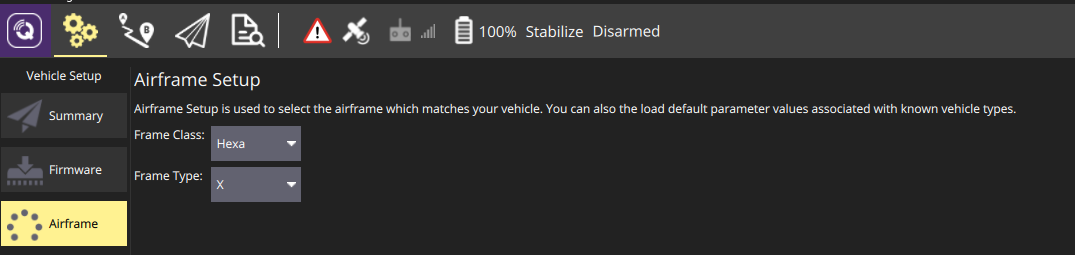
\includegraphics[width=\textwidth]{frame-setup.png}



\subsubsection{Radio Setup}
Die Auswahl der Flightmodie sowie die Kontrolle des Hexakopters erfolgt mithilfe einer \hyperlink{https://www.graupner.de/mediaroot/files/33124_mx20_HoTT_1_Web_DE.pdf}{Graupner mx 20} die der Pixhawk über den GR 16 Radio Empfänger anspricht (Siehe Kapitel \ref{Hardware Aufbau}).
Hierbei folge man zunächst einfach den Aufforderungen des \textbf{Calibrate} Dialogs.
%TODO wie Konfiguriert man die Knöpfe auf die Flightmodes ?

Die momentane Konfiguration ist mit Aufklebern auf der Fernbedienung markiert:

%TODO hier die Bilder der Fernbedienung einfügen
\subsubsection{flightmodes}
Die UAV kann in verschiedenen Flightmodes fliegen. Eine Liste der Verfügbaren Flightmodes findet sich hier: \hyperlink{http://ardupilot.org/copter/docs/flight-modes.html}{Arducopter-Flightmodes}.
Der Hexacopter ist bisher wie folgt konfiguriert:
\begin{figure}[H]
\centering
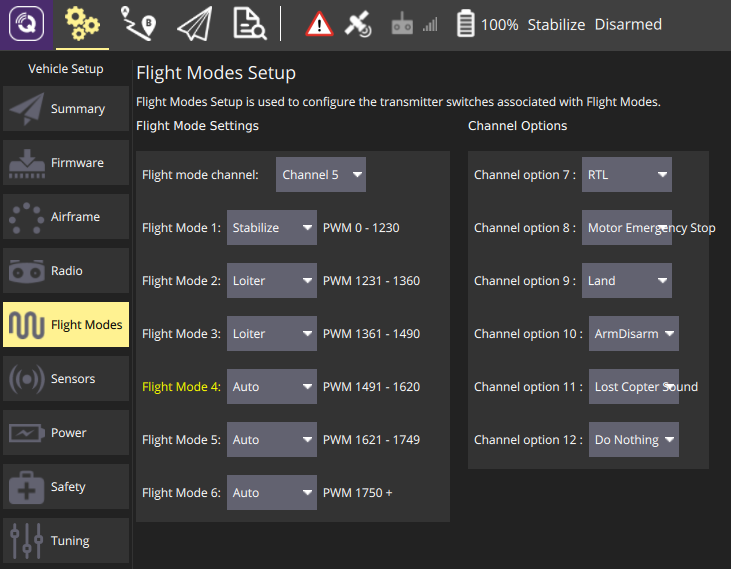
\includegraphics[width=0.7\textwidth]{flight-modes.png}
\end{figure}
\subsubsection{Sensors}
Um die Sensoren des Pixhawk zu Kalibrieren folge man der \hyperlink{https://docs.qgroundcontrol.com/en/SetupView/Sensors.html}{Dokumentation}
Es ist aber zu bemerken, das sich der Pixhawk zur Kalibrierung nicht auf dem Frame befinden muss, was diese erheblich erleichtert.
\subsubsection{Safety}
Unter dem Reiter \textbf{Safety} wurden folgende Einstellungen vorgenommen:
\begin{figure}[H]
\centering
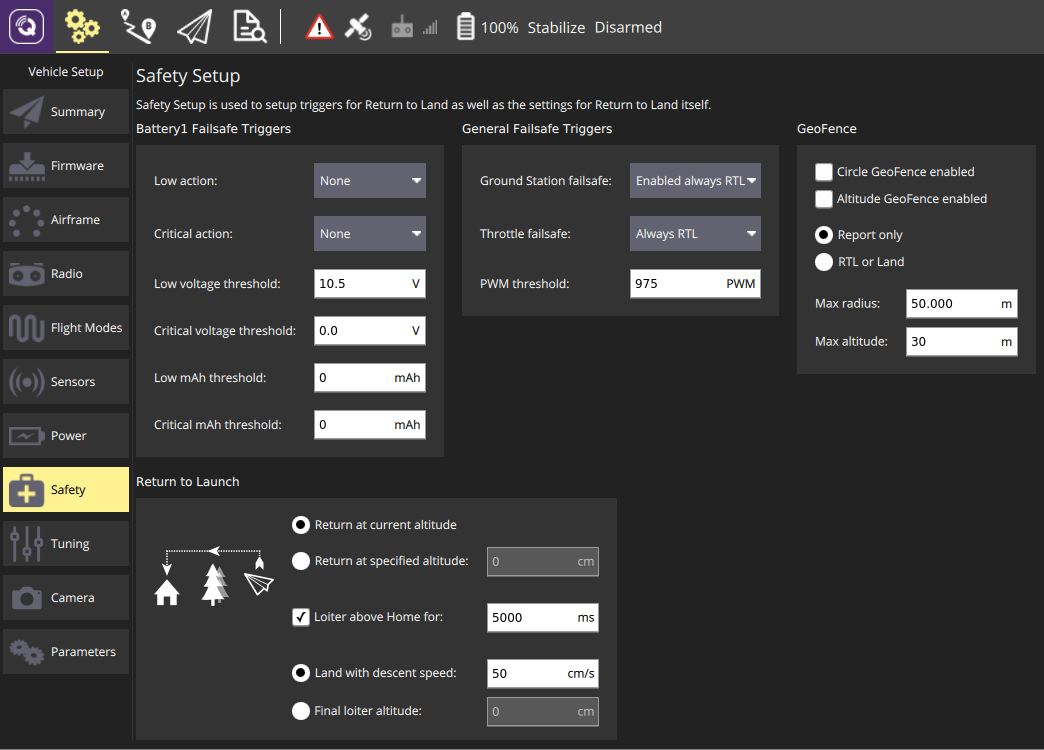
\includegraphics[width=\textwidth]{safety.png}
\end{figure}

\subsubsection{Parameters}
Damit der Raspberry Pi über Mavlink mit dem Flightcontroller Kommunizieren kann, wurden im Dialog \textbf{Parameters} folgende Einstellungen vorgenommen:
\begin{itemize}
\item SERIAL2\_PROTOCOL = 1
\item SERIAL2\_BAUD = 921600
\item LOG\_BACKEND\_TYPE = 3
\end{itemize}
Vergleiche hierzu die \hyperlink{http://ardupilot.org/dev/docs/raspberry-pi-via-mavlink.html}{Dokumentation}

\subsection{Raspberry Pi setup}
Der Raspberry Pi wurde mit dem \hyperlink{https://downloads.ubiquityrobotics.com/pi.html}{ubiquity image} (2018-11-15-ubiquity-xenial-lxde) geflasht.
Das Standartpasswort ist Ubuntu.
Auf dem Image ist bereits das komplette ROS Package sowie OpenCv installiert.
ROS wird außerdem automatisch gesourced sodass alle befehle direkt im Terminal verwendet werden können.
%TODO github setup beschreiben und aufzeigen wo sich die einzelnen Programme befinden
\subsection{Hardware Aufbau}

\subsubsection{Anschluss des ESC an die Motoren}
Die ESC wurde in der Mitte des Flamewheels auf Gummie-stüzten geschraubt, dazu mussten allerdings 4 Löcher in die untere Platte gebohrt werden, da nativ keine vorhanden wahren. Jeder der Ports wurde entsprechend des Folgenden Diagramms mit dem entsprechenden Motor verbunden.
Motornummer sollte außerdem dabei stehen.

\subsubsection{Anschluss des Pixhawk}
Bevor die Drone in Betrieb genommen werden kann, muss der \textbf{Hardware Safety Switch} mit dem GPS1 Port des Pixhawk verbunden werden, außerdem muss der Powerbrick an den POWER1 Port angeschlossen werden.
Optional kann auch der Buzzer per USB Port angeschlossen werden.
Der Anschluss der restlichen Komponenten ist der folgenden Abbildung zu entnehmen.
\begin{figure}[H]
\centering
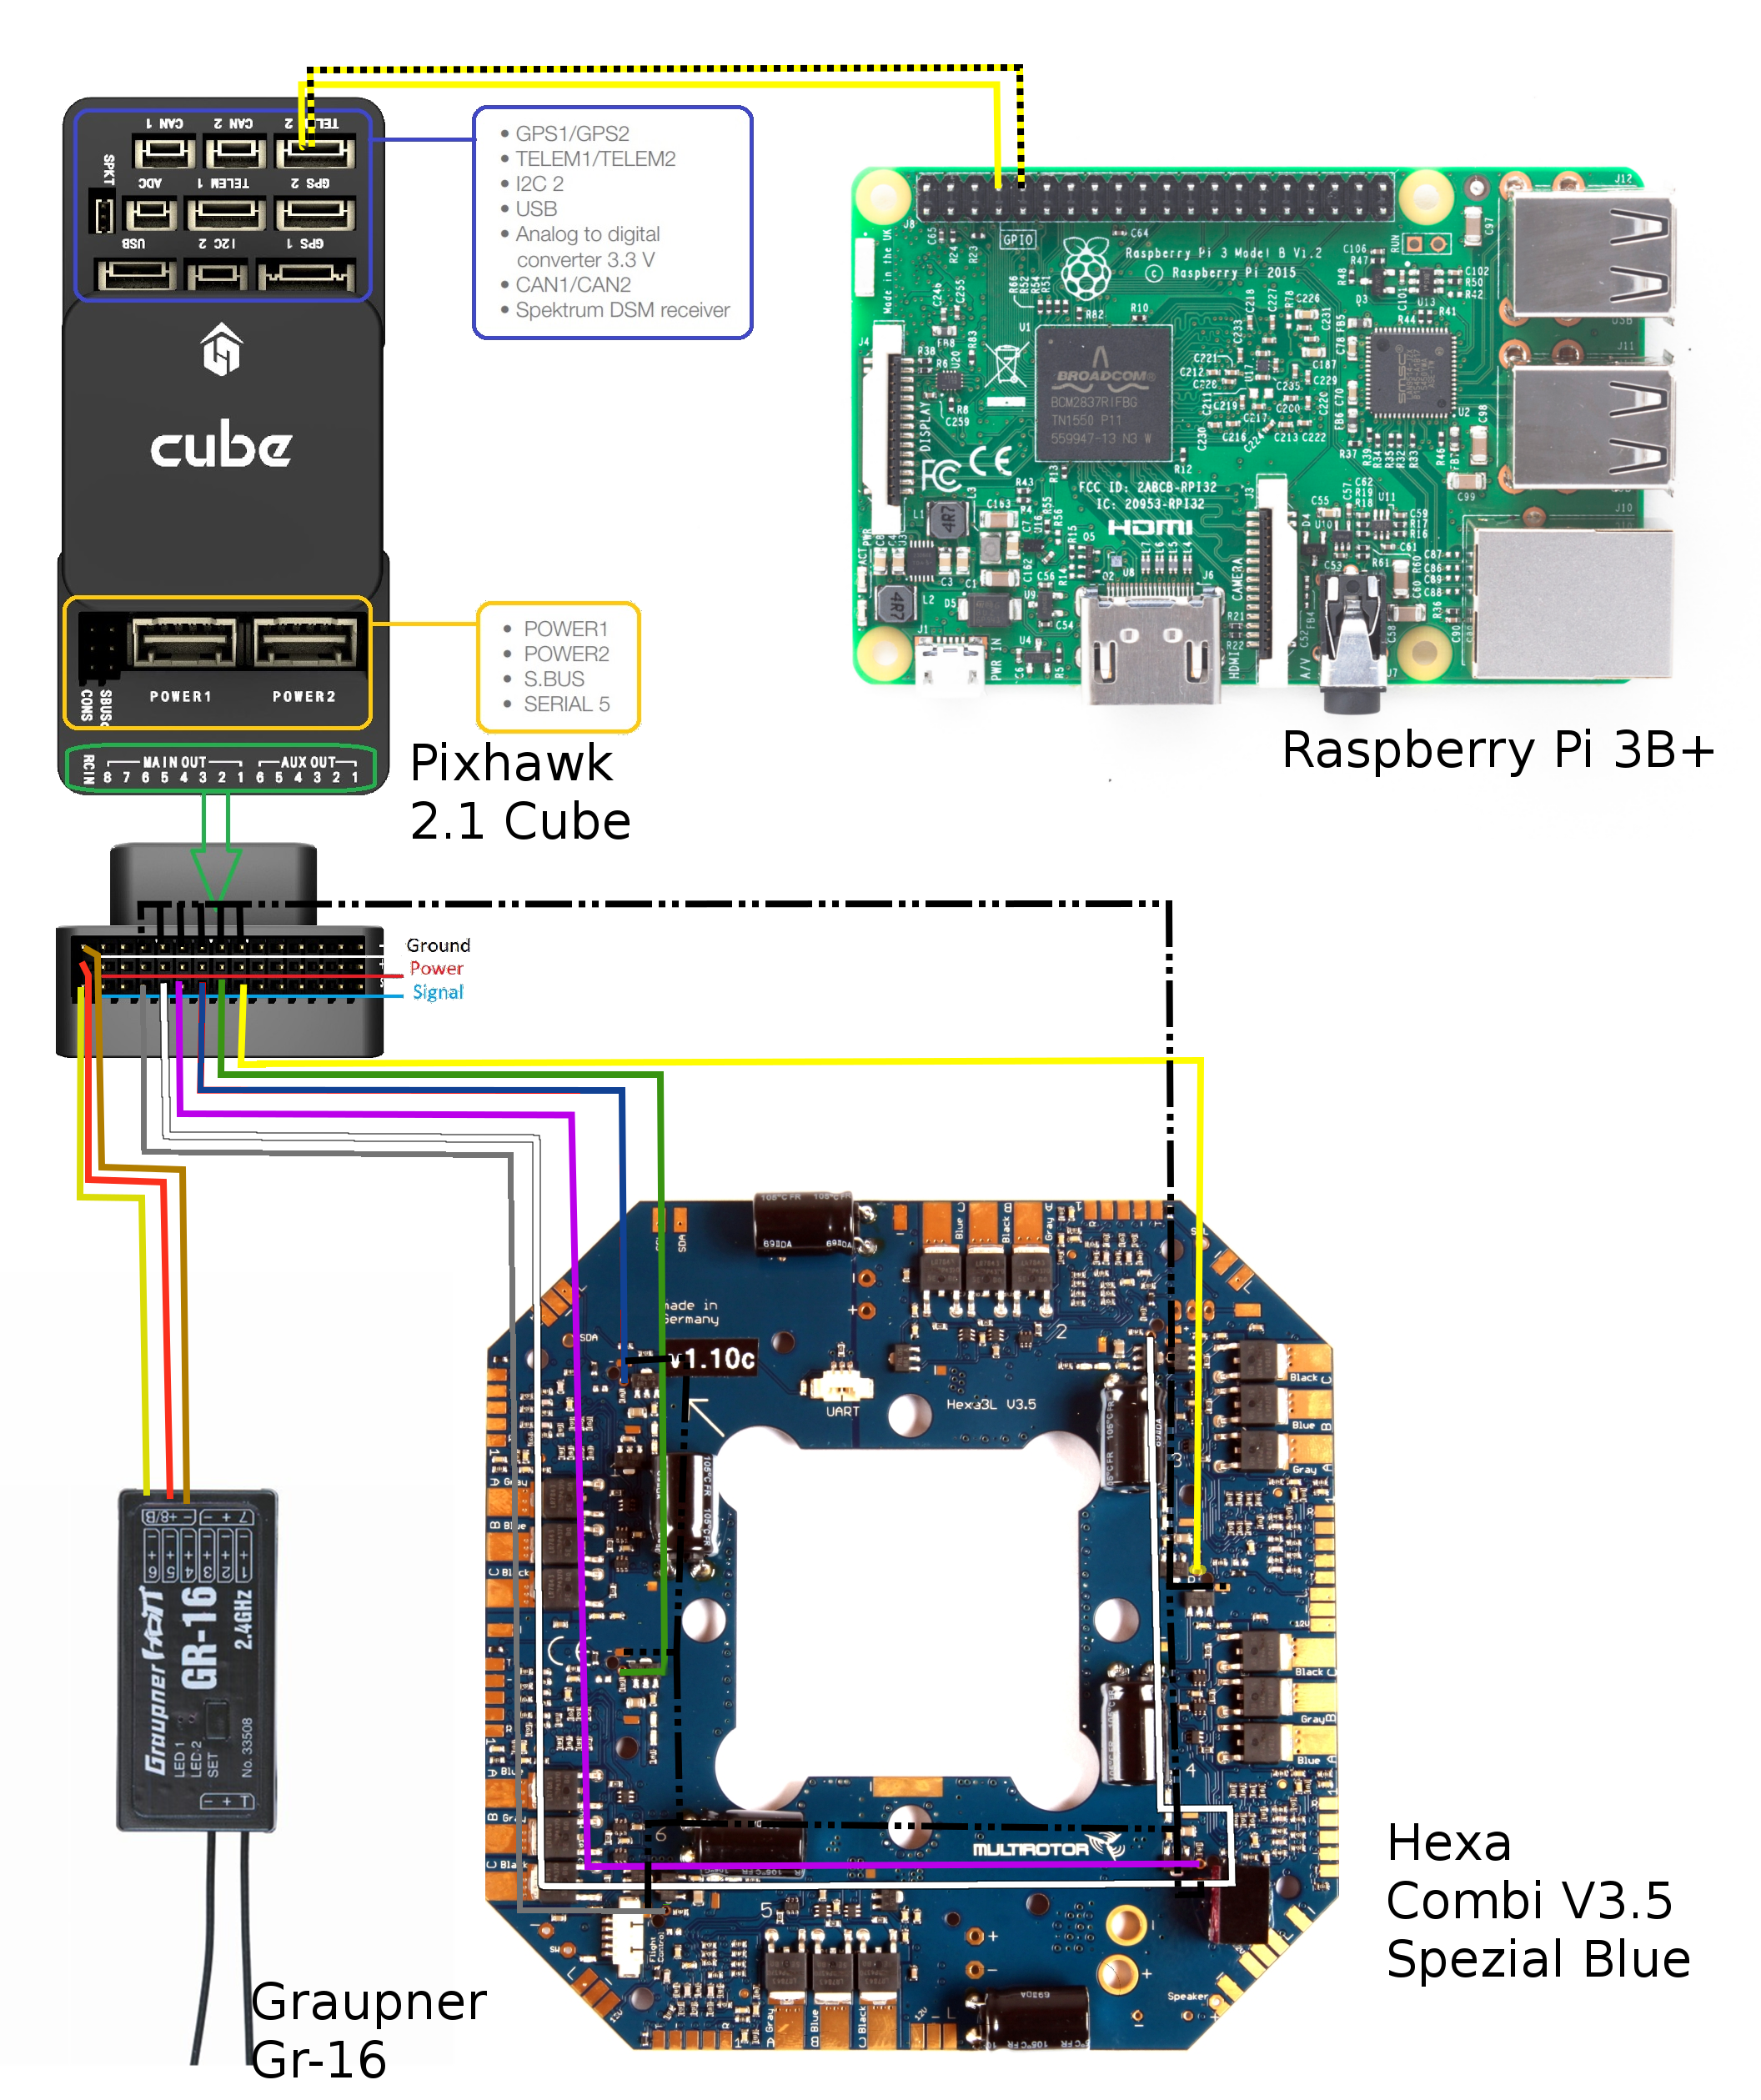
\includegraphics[width=\textwidth]{pixhawk-con.png}
\end{figure}

\subsubsection{Anschluss des Raspberry Pi}
Der Raspberry Pi wird von der selben Batterie gespeist mit der auch der Pixhawk betrieben wird.
Um dies zu ermöglichen muss zuerst das \hyperlink{http://downloads.joy-it.net/send/37-strompi-2/91-strompi-2-anleitung}{StromPi 2} Modul am Raspberry Pi befestigt werden. Je nachdem muss hier auch der Modus umgeschaltet werden, dafür folgt man einfach der oben verlinkten Anleitung.
\subsection{Starten des Hexacopters}

%TODO enumerate Syntax heraussuchen und in numerierte Liste verwandeln
\begin{enumerate}
\item  Fernbedienung anschalten

\item Flightcontroller-Batterie and Pixhawk Flight Controller und Raspberry Pi anschließen
%TODO hier Bild von connector einfügen
\item Motor-Batterie an ESC anschließen, dabei darauf achten das die Hände außer Reichweite der Propeller sind. Diese können manchmal nachdrehen.
%TODO wieder Bild einfügen
\item Den Rot Blinkenden Hardware Safety Switch drücken bis er konstant leuchtet.

\item den Arming Switch an der Fernsteuerung betätigen

\item  In den Flugmodus \textbf{Stabilizing} oder \textbf{Loitering} wechseln
\item  Den linken Stick der Fernsteuerung nach unten rechts drücken bis die Motoren angehen. Bei einer zulangen verzögerung zwischen 5 und 6 muss schritt 5 wiederholt werden. Ist ein Buzzer angeschlossen teilt dieser das disarming über ein piepen mit.

\item  Fliegen
\end{enumerate}

\subsection{Landen des Hexacopters}

\begin{enumerate}
\item UAV landen
\item Motor Batterie von ESC trennen
\item Flightcontroller Batterie von Pixhawk und Raspberry Pi trennen
\end{enumerate}

%TODO was ist mit automatischem Landen??



\end{document}


